\documentclass{ctexart}
\usepackage{amsmath}
\usepackage{graphicx}
\graphicspath{ {images/} }

\title{软件安全实验三 \ 恶意代码特征 }
\author{1181000420 韦昆杰}
\date{\today}

\begin{document}

\maketitle
\tableofcontents
\newpage

\section{实验项目描述}
面向网络恶意代码的特征提取

\subsection{理解基于最长公共子序列的协议特征提取方法}
\begin{enumerate}
  \item 掌握网络恶意代码特征的提取流程
  \item 学习最长公共子序列的提取算法
\end{enumerate}

\subsection{实现字符串最长公共子序列的提取算法}
\begin{enumerate}
  \item 利用动态规划的方法实现字符串最长公共子序列的提取
  \item 依据输入的字符串构建L(m,n)数组,利用L(m,n)数组查找两个字符串之间的最长公共子序列
\end{enumerate}


\section{实验要求}
\begin{enumerate}
  \item 实验数据准备。利用ASCII字符集做为输入集,不考虑多字节编码的中文、英文字符集。
  \item 程序的输入部分:2个字符串。输出部分:这2个字符串的最长公共子序列,如有多个一同给出。
  \item 实验结果和实验数据一起给出。
\end{enumerate}

\section{实验结果}
\subsection{设计的算法流程图,以及算法说明}

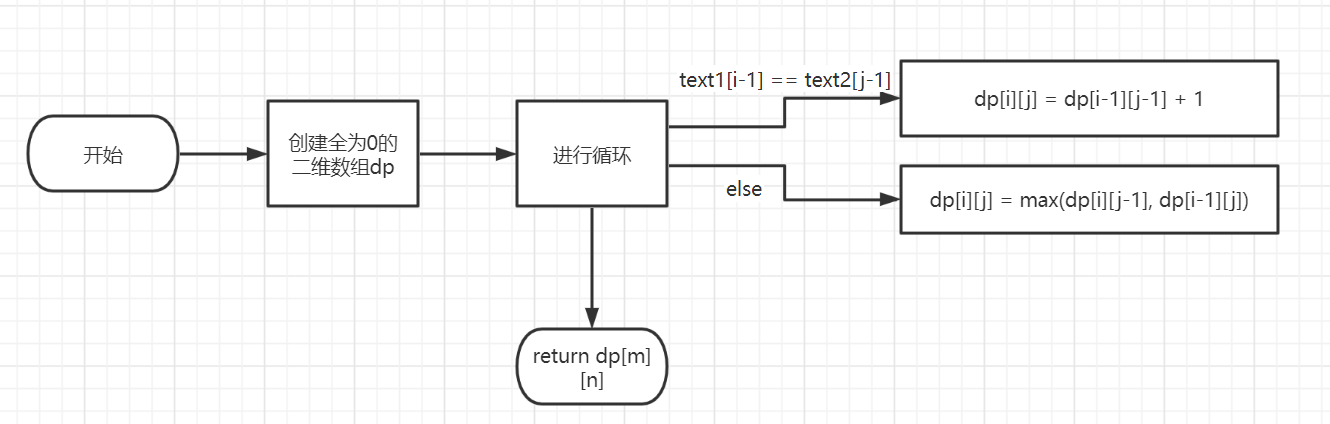
\includegraphics[width=\textwidth]{diagram.png}

算法说明:
\newline

设$X = (x1,x2...x_m)$ 和 $Y=(y1,y2...y_n)$ 是两个序列,将 X 和 Y 的最长公共子序列记为$LCS(X,Y)$,可得以下公式

设 X=(x1,x2,.....xn) 和 Y={y1,y2,.....ym} 是两个序列,将 X 和 Y 的最长公共子序列记为LCS(X,Y),从X和Y的最后一个字符开始比较,可知
\[ 
LCS(X_i,Y_j)=
\begin{cases}
0, &  if \ \ i=0  \ or  \ j=0   \\
LCS(X_{i-1},Y_{j-1})+1, & if \ \ i,j>0  \ and  \ x_i=y_i   \\
max(LCS(X_i,Y_{j-1}),LCS(X_{i-1},Y_j)), & if \ \ i,j>0  \ and  \ x_i \neq y_i   
\end{cases}  
\]

\subsection{关键的数据结构,及简单说明}

二维数组dp,假设2个字符串分别为s1和s2,那么dp[i][j]代表s1[0:i]和s2[0:j]的最长公共子序列的长度

二维数组res,res[i][j]表示s1[0:i]和s2[0:j]的最长公共子序列

最终返回结果是res[m][n],m为s1的长度,n为s2的长度

\subsection{实验结果的截图}
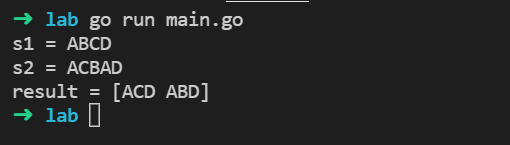
\includegraphics[width=\textwidth]{result.png}

\subsection{源程序}
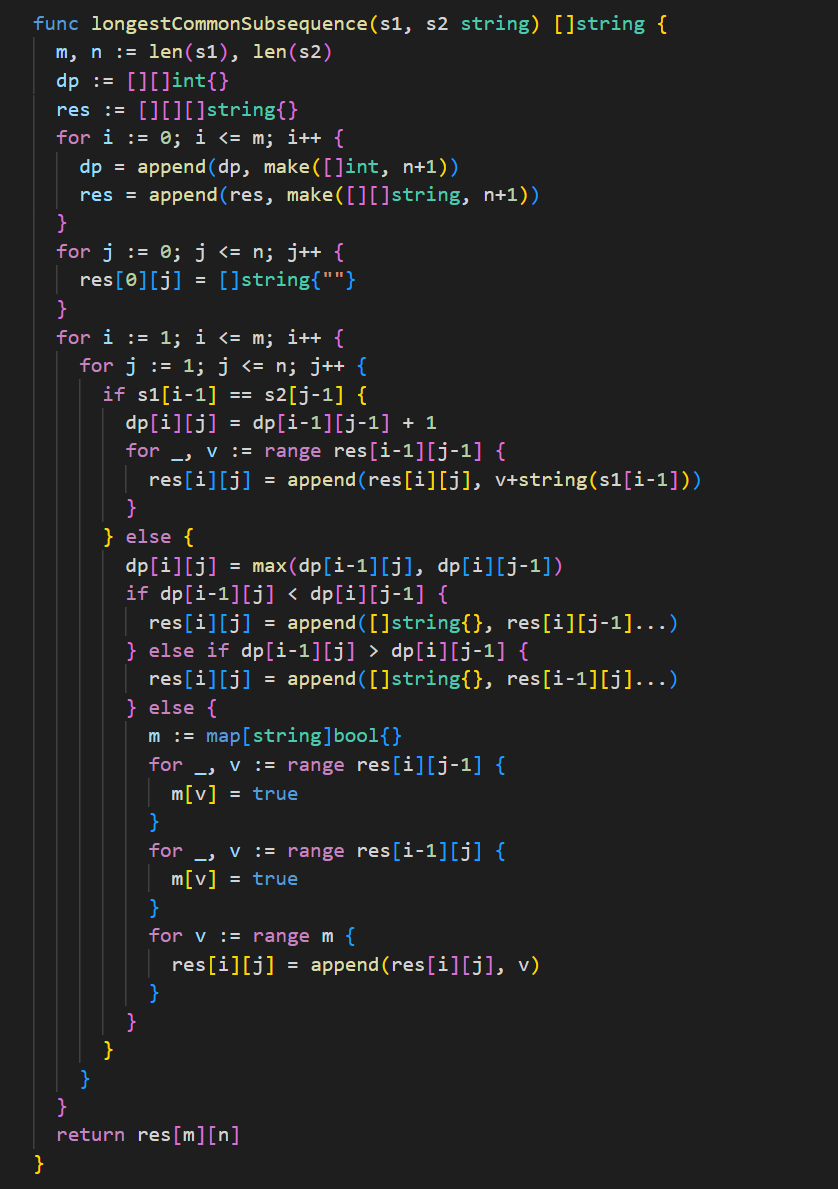
\includegraphics[width=\textwidth]{code.png}

\end{document}